
%%%%%%%%%%%%%%%%%%%%%%%%%%%%%%%%%%%%%%%%%%%%%%%%%%%%%%%%%%%%%%%%%%%%%%%%%%%%%%%%%%%%%%%
%%%%%%%%%%%%%%%%%%%%%%%%%%%%%%%%%%%%%%%%%%%%%%%%%%%%%%%%%%%%%%%%%%%%%%%%%%%%%%%%%%%%%%%
% 
% This top part of the document is called the 'preamble'.  Modify it with caution!
%
% The real document starts below where it says 'The main document starts here'.

\documentclass[12pt]{article}

\usepackage{amssymb,amsmath,amsthm}
\usepackage[top=1in, bottom=1in, left=1.25in, right=1.25in]{geometry}
\usepackage{fancyhdr}
\usepackage{enumerate}
\usepackage{listings}
\usepackage{graphicx}
\usepackage{float}

\usepackage{mwe}
\usepackage{caption}
\usepackage{subcaption}
% Comment the following line to use TeX's default font of Computer Modern.
\usepackage{times,txfonts}



\makeatletter
\renewcommand*\env@matrix[1][*\c@MaxMatrixCols c]{%
  \hskip -\arraycolsep
  \let\@ifnextchar\new@ifnextchar
  \array{#1}}
\makeatother

\newtheoremstyle{homework}% name of the style to be used
  {18pt}% measure of space to leave above the theorem. E.g.: 3pt
  {12pt}% measure of space to leave below the theorem. E.g.: 3pt
  {}% name of font to use in the body of the theorem
  {}% measure of space to indent
  {\bfseries}% name of head font
  {:}% punctuation between head and body
  {2ex}% space after theorem head; " " = normal interword space
  {}% Manually specify head
\theoremstyle{homework} 

% Set up an Exercise environment and a Solution label.
\newtheorem*{exercisecore}{Exercise \@currentlabel}
\newenvironment{exercise}[1]
{\def\@currentlabel{#1}\exercisecore}
{\endexercisecore}

\newcommand{\localhead}[1]{\par\smallskip\noindent\textbf{#1}\nobreak\\}%
\newcommand\solution{\localhead{Solution:}}

%%%%%%%%%%%%%%%%%%%%%%%%%%%%%%%%%%%%%%%%%%%%%%%%%%%%%%%%%%%%%%%%%%%%%%%%
%
% Stuff for getting the name/document date/title across the header
\makeatletter
\RequirePackage{fancyhdr}
\pagestyle{fancy}
\fancyfoot[C]{\ifnum \value{page} > 1\relax\thepage\fi}
\fancyhead[L]{\ifx\@doclabel\@empty\else\@doclabel\fi}
\fancyhead[C]{\ifx\@docdate\@empty\else\@docdate\fi}
\fancyhead[R]{\ifx\@docauthor\@empty\else\@docauthor\fi}
\headheight 15pt

\def\doclabel#1{\gdef\@doclabel{#1}}
\doclabel{Use {\tt\textbackslash doclabel\{MY LABEL\}}.}
\def\docdate#1{\gdef\@docdate{#1}}
\docdate{Use {\tt\textbackslash docdate\{MY DATE\}}.}
\def\docauthor#1{\gdef\@docauthor{#1}}
\docauthor{Use {\tt\textbackslash docauthor\{MY NAME\}}.}
\makeatother

% Shortcuts for blackboard bold number sets (reals, integers, etc.)
\newcommand{\Reals}{\ensuremath{\mathbb R}}
\newcommand{\Nats}{\ensuremath{\mathbb N}}
\newcommand{\Ints}{\ensuremath{\mathbb Z}}
\newcommand{\Rats}{\ensuremath{\mathbb Q}}
\newcommand{\Cplx}{\ensuremath{\mathbb C}}
%% Some equivalents that some people may prefer.
\let\RR\Reals
\let\NN\Nats
\let\II\Ints
\let\CC\Cplx
%%%%%%%%%%%%%%%%%%%%%%%%%%%%%%%%%%%%%%%%%%%%%%%%%%%%%%%%%%%%%%%%%%%%%%%%%%%%%%%%%%%%%%%
%%%%%%%%%%%%%%%%%%%%%%%%%%%%%%%%%%%%%%%%%%%%%%%%%%%%%%%%%%%%%%%%%%%%%%%%%%%%%%%%%%%%%%%
% 
% The main document start here.

% The following commands set up the material that appears in the header.




%  \textbf{Code:}
%  \begin{center}
%  \lstinputlisting[basicstyle = \footnotesize]{}
%  \end{center}
%  
%  \begin{footnotesize}
%  \begin{verbatim}
%    
%  \end{verbatim}
%  \end{footnotesize}
%  
%  
%  \begin{figure}[H]
%    \begin{center}
%      \caption{}
%    \includegraphics[width = \textwidth]{}
%    \end{center}
%  \end{figure}




\doclabel{Stat 461: Homework 6}
\docauthor{Stefano Fochesatto}
\docdate{\today}

\begin{document}
\begin{exercise}{1} Read the data in the appendix into R. You will examine the data in 3d:
  \begin{footnotesize}
  \begin{verbatim}
    library(car)
    library(car)
    scatter3d(x1~x2+x3, data=dat, neg.res.col="white",
    pos.res.col="white", surface.alpha=0.0)
  \end{verbatim}
  \end{footnotesize}
  \begin{enumerate}
    \item[a.] Use kmeans to determine the optimal number of clusters, and then plot the 3d plot.\\
    \solution The kmeans algorithm simply finds the optimal partition of the data which reduces the intra-class variance (sum of squared distances from cluster 
    centroids). With that in mind determining an optimal number of clusters is subjective, however we can make an informed decision on how many clusters we should use 
    by examining the ratio between the sum of squares between clusters and the sum of squares total (like $r^2$). The greater this ratio, the more of the variance is explained by our clustering.
    Simulating kmeans for 1 to 10 clusters and computing the $r^2$ we get the following, 
      \begin{figure}[H]
        \begin{center}
          \caption{Plot of $r^2$ up to 10 Clusters.}
        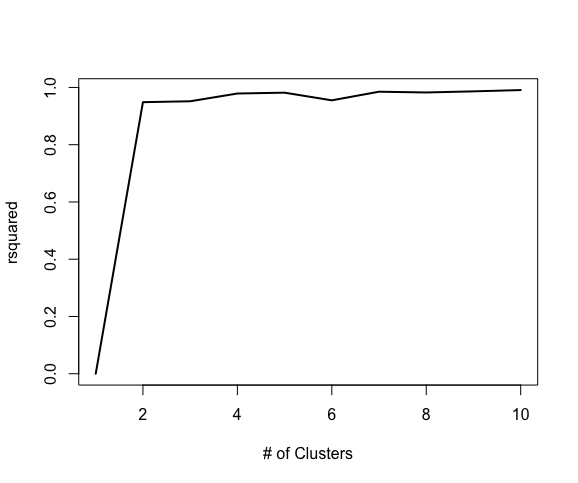
\includegraphics[width = .65\textwidth]{Rplot01.png}
        \end{center}
      \end{figure}
      Clearly we can see that after 2 clusters we are seeing marginal returns on the amount of variance explained. 
      Comparing the 2 clustering and the data, it seems as though 2 clusters is satisfactory, and likely the true signal behind whatever system 
      generated the data. 
        \begin{figure}[H]
          \begin{center}
            \caption{3D Data Plot}
          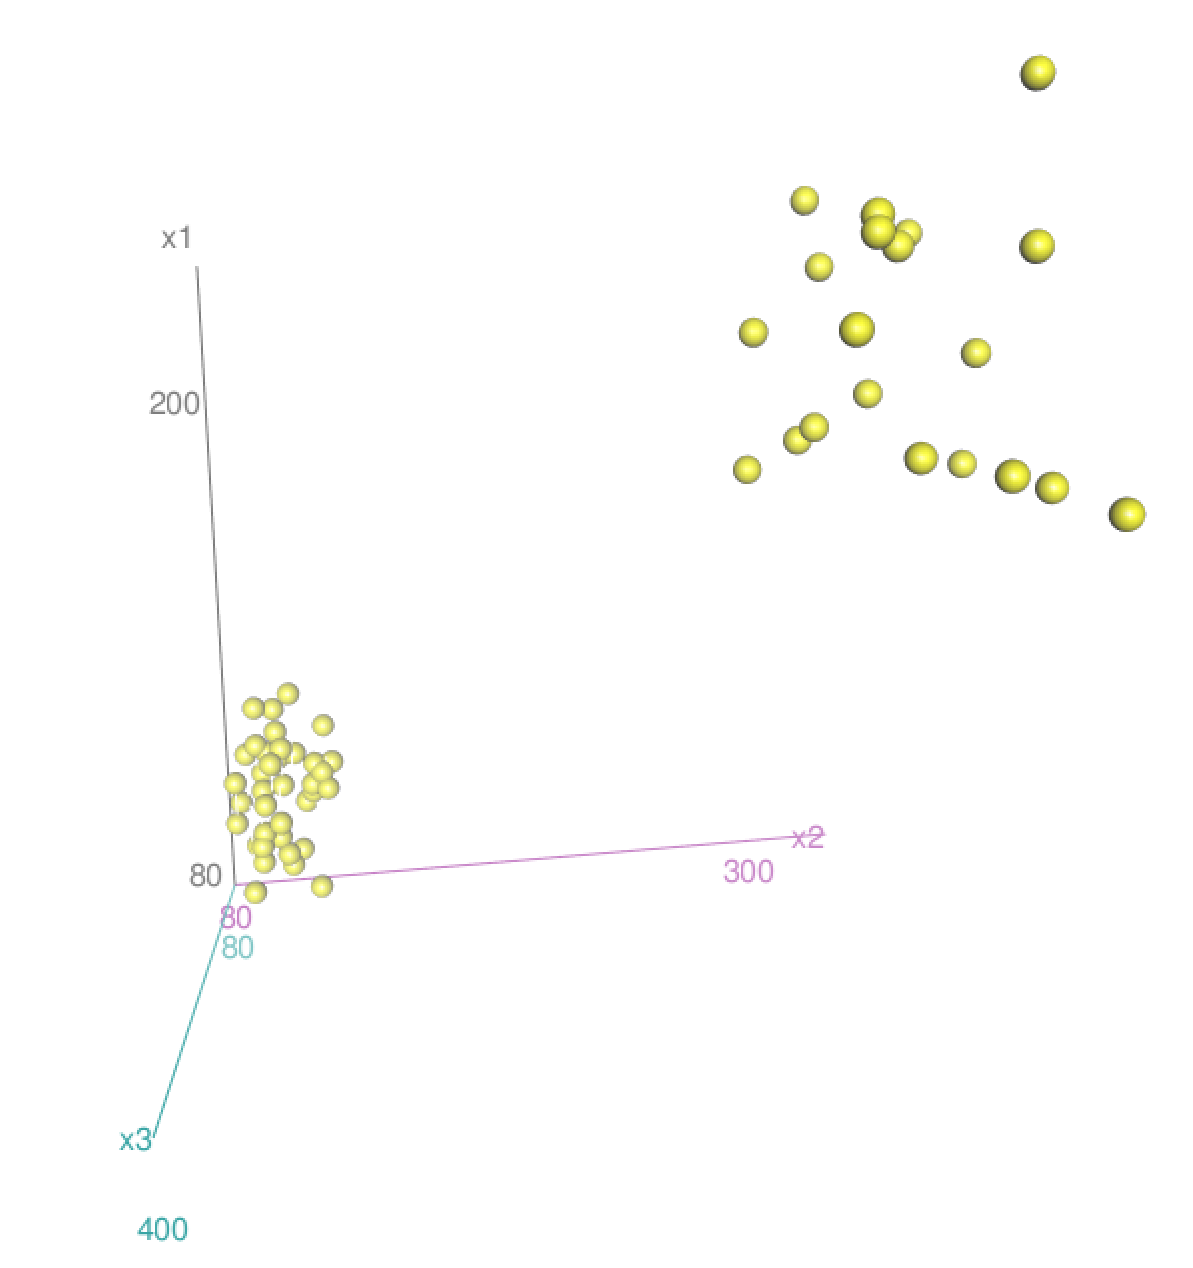
\includegraphics[width = .80\textwidth]{Dat3d.png}
          \end{center}
        \end{figure}
        \begin{figure}[H]
          \begin{center}
            \caption{3D Data Plot With 2 Clusters}
          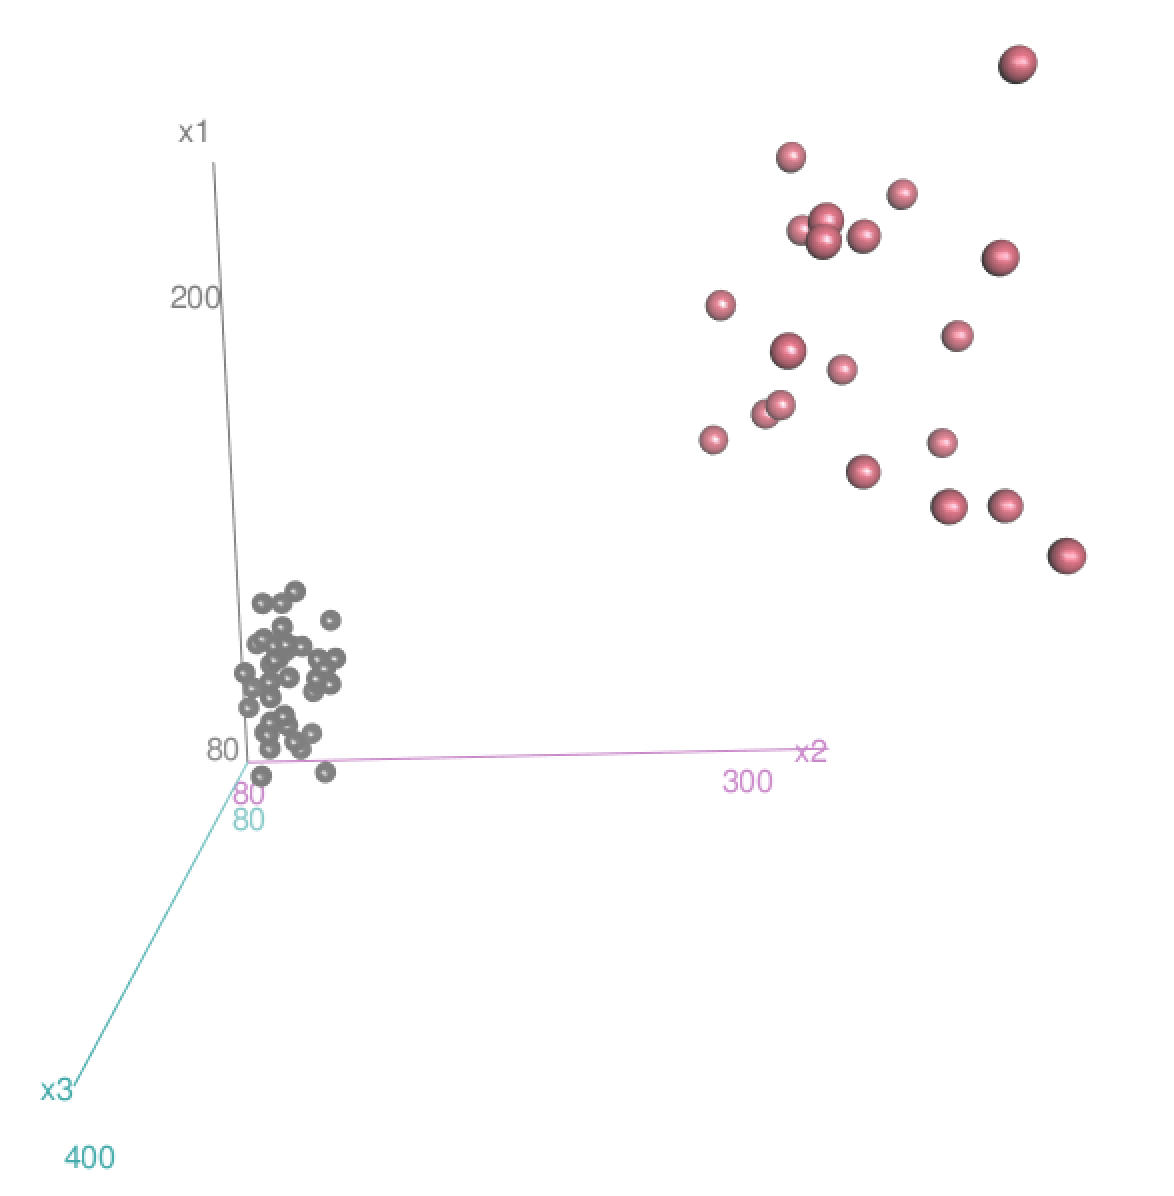
\includegraphics[width = .80\textwidth]{Dat3DClustered.png}
          \end{center}
        \end{figure}
        \vspace{.15in}



      \item[b.] Now use a hierarchical method. Try both complete and single linkage. Do you get the same clustering in the same order for both linkages?\\
      \solution Using an agglomerative hierarchical method with the hclust() function we got the following dendrograms for the given data, using both linkages and euclidean distances,
      \begin{figure}[H]
        \begin{center}
          \caption{Single Linkage}
        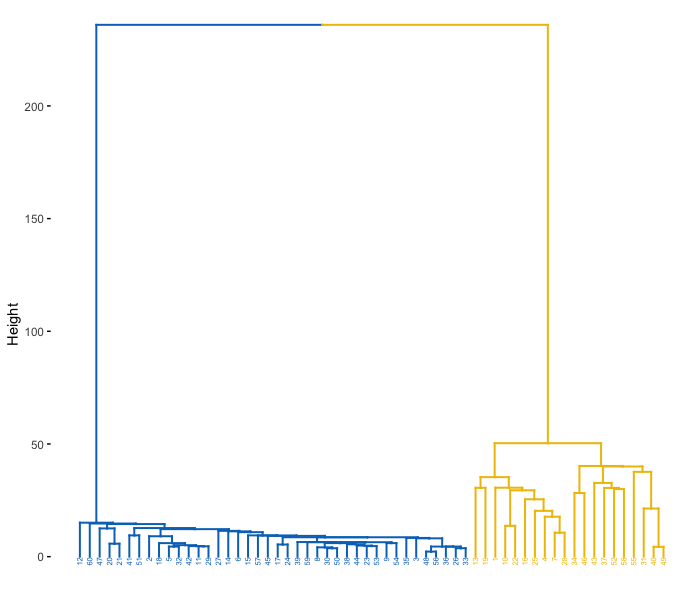
\includegraphics[width = .70\textwidth]{Rplot.png}
        \end{center}
      \end{figure}
      \begin{figure}[H]
        \begin{center}
          \caption{Complete Linkage}
        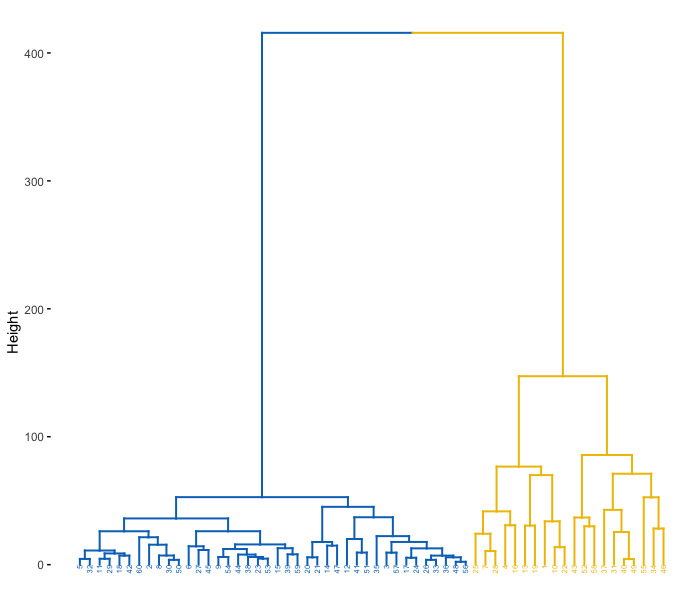
\includegraphics[width = .70\textwidth]{Rplot02.png}
        \end{center}
      \end{figure}
      The following figure shows that each clustering method resulted in the same clusters, however using the order call on the dendrogram object we can see that the order is not the same, 
      \begin{figure}[H]
        \begin{center}
          \caption{Checking Clusters}
        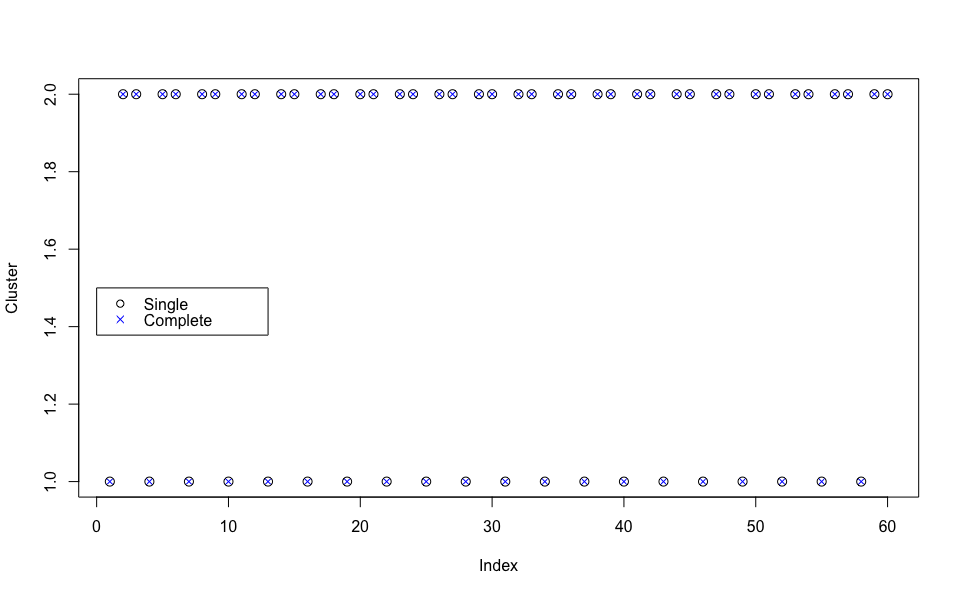
\includegraphics[width = \textwidth]{Rplot03.png}
        \end{center}
      \end{figure}

        \textbf{Code:}
        \begin{center}
        \lstinputlisting[basicstyle = \footnotesize]{r2.txt}
        \end{center}
        \vspace{.15in}



        \item[c.] What is complete linkage? What is single linkage?\\
        \solution Linkage describes how we measure distance between clusters (and clusters and single observations). Suppose $A$ and $B$ are clusters such that 
        $x \in A$ and $y \in B$ then under single linkage we get the following, 
        \begin{equation*}
          d(A,B) = min(x, y).
        \end{equation*}
        Under complete complete linkage we get the following, 
        \begin{equation*}
          d(A,B) = max(x, y).
        \end{equation*}

  \end{enumerate}

\end{exercise}
\vspace{.15in}

\begin{exercise}{2}
  \begin{enumerate}
    \item[a.] Import the Woody Species data set.\\ 
    \solution 
    \textbf{Code:}
    \begin{center}
    \lstinputlisting[basicstyle = \footnotesize]{r3.txt}
    \end{center}
    \vspace{.15in}
    
    \item[b.] Now use kmeans to determine a 'reasonable' number of clusters. You should justify your choice of cluster numbers.\\
    \solution Generating the $r^2$ plot similarly to the first problem we get the following plots, 
    \begin{figure}[H]
      \begin{center}
        \caption{Plot of $r^2$ up to 10 Clusters.}
      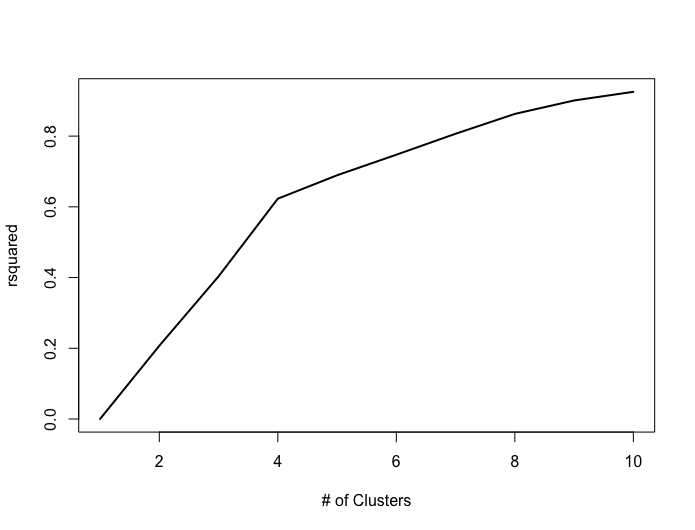
\includegraphics[width = .70\textwidth]{Rplot04.png}
      \end{center}
    \end{figure}
    \begin{figure}[H]
      \begin{center}
        \caption{Proportion of $r^2$ for Each Cluster.(Scree-ish plot)}
      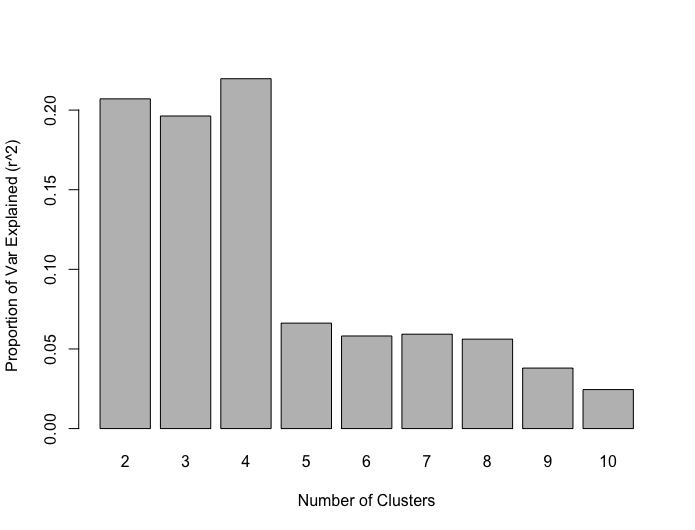
\includegraphics[width = .70\textwidth]{Rplot05.png}
      \end{center}
    \end{figure}
    From here we can see that adding the fifth cluster contributes, marginally to the proportion of variance explained, and therefore I would explore clustering into 4
    or less groups. \\
    \textbf{Code:}
    \begin{center}
    \lstinputlisting[basicstyle = \footnotesize]{r4.txt}
    \end{center}
    \vspace{.15in}


    \item[c.] Briefly, how does kmeans() work?\\
    \solution The kmeans algorithm begins by randomly assigning the data to $n$(hyperparameter) different clusters. Then the centroid of each cluster is computed. 
    The data are reassigned to the same cluster as the nearest centroid. New centroids are computed and the data is reassigned again recursively. Eventually this algorithm 
    converges, and sometimes it shows sensitivity to initial conditions which is why kmeans() runs several randomized instances of this algorithm.
  \end{enumerate}
  \vspace{.15in}


  \item[d.] Now cluster the data using any hierarchical clustering method you wish. Don't forget to think about a reasonable distance measure. Do you get similar clusters to when you used kmeans?\\
   

  
\end{exercise}









\end{document}


















